\chapter{Interfacing with LLDB\label{cha:chapter4}}

%todo refactor

We developed the first prototype of a native debugger for OCaml, based on the LLDB debugging framework on top of LLVM. For that, we first generated a full OCaml binding for the LLDB library, by parsing the C++ headers of the libraries and automatically generating OCaml and C++ stubs. We were then able to use the OCaml binding to develop several tools, ranging from a simple tool that displays the internal GC information of a finished OCaml application, to an almost complete debugger, which displays OCaml values using runtime type information added for memory profiling.

The OCaml native runtime system
LLDB (API)
ocp(lib)-lldb (hl archi)

additions to LLDB and ocp-lldb

\section{Introduction to LLDB}

LLDB\autocite{lldb}
aims to be a modern source-level debugger, modular plug-in arch (for obj file
format, prog lang support, symbol files, disasm, specific hosts/targets), reusable components, public
C++ API interface to library for access to and control of debugger instances,

python bindings,
can interact with debug instances and build applications that provide debugging features

 C, Objective-C, C++ Swift

part of the llvm project (collection of compiler tools with reusable components)
including clang compiler prog lang frontend, and llvm middle end IR and code gen backends
for multiple architectures, machine dependent? target

several compiler frontends for support of mult prog languages (clang, rust)


Figure \ref{fig:aliceandbob} illustrates the situation between Alice and Bob. (sequence diagram from www.websequencediagrams.com)


\subsection{LLDB OCaml language plugin}

at this point, a OCaml program compiled with a compiler and modifications
presented previously contains more information relevant to debugging than before

more places where to set a breakpoint in the program
runtime location of variables
type information

however, the information provided by 2 and 3 cannot be used directly as it is yet:
using LLDB directly


current versions of LLDB arent aware of OCaml
Ocaml binary mixing C with OCaml assembly code
LLDB bindings doesnt allow access to the DWARF data nor name symbol demangling

however, it is now possible for LLDb to support other languages/ debug binaries
written in different programming languages
% depuis un peu moins d'un an, chgmts faits a LLDB pour pouvoir supporter d'autres languages que ceux supportes par clang
% il suffit d'ecrire des classes impl certaines interfaces
% ajouter le language cible dans un enum

% eventuellement pouvoir evaluer expr dans ce language
% pretty printing des valeurs et typage dynamique, ptes statiques ou dyn du language
facilities for evaluating language expressions
express static dynamic properties of the language

among the addition done to LLDB

barebones OCaml LLDB plugin

custom DWARF parser

minimal type system, data structures used to represent OCaml types may
    change from one version to another, it might not be maintainable to update
    the LLDB plugin at each release
    backwards compatibility concerns
    thus, all values are to be considered as 64-bits integers, and their
    interpretation according to their types will be left to ocp-lldb

    does symbol demangling as well

    mangled ocaml symbol of the form
    make demangled form available for easier breakpoint setting

\section{ocp-lldb}

%todo ocp-lldb architecture


\begin{figure}
  \centering
\begin{tikzpicture}[node distance=3pt,outer sep=0pt,
blueb/.style={
  draw=white,
  fill=mybluei,
  rounded corners,
  text width=2.5cm,
  font={\sffamily\bfseries\color{white}},
  align=center,
  text height=12pt,
  text depth=9pt},
greenb/.style={blueb,fill=mygreen},
]
\node[blueb] (ocl) {ocp-lldb};
%\node[blueb,right=of RCP] (Aut) {Authoring};
%\node[blueb,right=of Aut] (Bro) {Browsing};
\node[blueb,below=of ocl] (ocll) {ocplib-lldb};
\node[blueb,below=of ocll] (lldb) {liblldb};
\node[blueb,fill=mypink,below=of lldb] (bin) {OCaml binary};
\node[left=of bin] (asrs) {Output};
\end{tikzpicture}
\end{figure}

%\begin{figure}[htb]
  %\centering
  %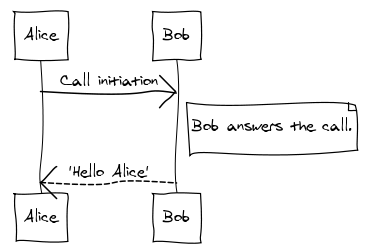
\includegraphics[width=9cm]{uml_seq_example.png}\\
  %\caption{Alice and Bob}
  %\label{fig:aliceandbob}
%\end{figure}

ocplib-lldb \\

taking advantage of the OCaml compiler frontend as a library
allowing use of the lexer and parser and typing facilities, esp
useful when operating over parsetree/typedtree representation

used to build symbol table mapping identifiers in the prog to their type
for runtime value interpretation

can generate an OCaml binding to LLDB API

parse header files in LLDB
most classes and methods of the API are supported, except static methods
access to C++ objects done through the OCaml FFI C interface

ocp-lldb

symbol table management :
read the serialized typed AST, iterate over it to extract a simpler tree
structure
then one can actually lookup the type associated with an identifier and display
its value accordingly

for the moment, can print the following types:

\section{Runtime memory representation of OCaml values}

all values represented as a single word (of either 32 or 64 bits)

to differentiate between pointers and integer values at runtime, the runtime
system uses a tagged pointer representation, the least significant bit of a
value is used as a tag : an OCaml integer is encoded as a 31 or 63-bit integer = $ (x \ShiftLeft 1) \BitOr 1 $

mere integers are not boxed, the tag bit will be set to one
as for pointers, since they are word-aligned, their tag bit will be set to zero
(they are multiples of 4, therefore they will always end with two 0 bits)

\Glspl{boxed} are represented as a single word pointer to a block structure, made of a
header followed by data
The header contains metadata about the value such as size of the block, and tag describing what type of data it
contains
add level of indirection / deref


int, char are unboxed
unit, false, empty list [] as 0
true as 1

arrays, records, tuples -> header + array of values
records with floats fields, array of floats -> header + array of floats

variant types -> variants without paramter are unboxed ascending ints, non
constants variants with parameters are boxed
